\documentclass[11pt]{article}
\usepackage[left=2cm, top=1.5cm, right=2cm, bottom=1.5cm]{geometry}
\usepackage[utf8]{inputenc}
\usepackage[T1]{fontenc}
\usepackage[french]{babel}
\usepackage{graphicx}
\usepackage{graphics}
\usepackage{amsmath}
\usepackage{tikz}
\usepackage{xcolor} 
\usepackage{mathtools}
\usepackage{parskip}
\usepackage{subcaption}
\usepackage[export]{adjustbox}
\usepackage{multicol}

\title{\vspace{-2cm}\textbf{TP 5 - Induction électromagnétique}}
\author{\vspace{-0.5cm}MENARD Alexandre - VIEILLEDENT Florent}
% \setlength{\parindent}{1cm}
\date{\vspace{-0.7cm}}


\newcommand{\ut}{\vec{u_\theta}}
\newcommand{\ur}{\vec{u_r}}
\newcommand{\uz}{\vec{u_z}}

\begin{document}
\maketitle

En présence d'un champ magnétique variable, un circuit électrique voit apparaître une tension à ses bornes, on parle d'induction électromagnétique.
Ce phénomène est aujourd'hui utilisé dans la charge par induction des smartphones, mais aussi dans les alternateurs et transformateurs électriques.
Dans ce travail pratique, nous proposons une étude qualitative et quantitative de la loi de Lenz-Faraday afin de vérifier sa cohérence avec l'expérience. 
Enfin, nous étudierons des transformateurs de tension, important pour optimiser le transport d'énergie électrique dans les réseaux.

\section{Loi de Lenz-Faraday en champ variable}
\subsection{Théorie}
Dans le cadre de ce travail pratique, nous nous placerons dans l'approximation des régimes quasi-stationnaires, le courant
sera donc le même partout dans un même circuit, et l'on négligera les temps de propagation du champ magnétique entre les deux circuits.
Soit 2 bobines de diamètre $d$ et de nombre de spires $N_H$ placées à une distance $d/2$ l'une de l'autre, et parcourues par un courant $i(t) = i_0\sin(\omega t + \psi)$.	
On a alors le flux magnétique au travers d'une bobine à section carré de côté $a \in [a_{min}, a_{max}]$ :
\begin{align}
    \label{eqn:relation_1}
    \Phi(t) & = \overbrace{\left(\frac{4}{5} \right)^{\frac{3}{2}} \frac{2\mu_0 N_H}{d}}^{\alpha} \overbrace{\left(\frac{a_{min}^2 + a_{max}^2 + a_{min}a_{max}}{3}\right)}^{S} N \cos \theta i(t) \nonumber\\
    & = \alpha S N i(t)
\end{align}
On en déduit alors la force électromotrice induite (f.e.m) dans la bobine carrée:
\begin{align}
    e(t) = -\frac{d\Phi(t)}{dt} = -\alpha S N \omega \cos \theta i_0 \cos (\omega t + \psi) = \alpha S N \omega \cos \theta i_0 \sin (\omega t + \psi - \frac{\pi}{2})
\end{align}

On s'attend alors à ce que le déphasage entre $e(t)$ et $i(t)$ soit de $\frac{\pi}{2}$, avec $e(t)$ qui sera en retard. Enfin, $e(t)$ est proportionnel
à $N$, $\omega$ et $\cos \theta$.

Enfin, pour déterminer l'inductance mutuelle $M$, on a:
\begin{align}
  \label{eqn:relation_M}
  \frac{e}{i} = \alpha S N \omega \text{ et } M = \frac{\Phi_{1 \rightarrow 2}}{ i} = \alpha S N \Rightarrow \frac{e}{i} = M \omega
\end{align}

\subsection{Montage expérimental et détermination des incertitudes}
\label{section:protocole}
On installe 2 bobines de Helmholtz de diamètre $d = 13cm$, avec $N_H = 95 spires$, que l'on sépare d'une distance $d/2$. On les installe en série sur la sortie
à $50\Omega$ d'un GBF, puis en sortie de la dernière, on relie à l'oscilloscope, puis l'on termine le circuit sur la masse de la sortie du GBF. 
On installe ensuite au centre des deux bobines, une troisième bobine dite inductive de section $S$ (voire (\ref{eqn:relation_1})) dont on relie les bornes à l'oscilloscope.

Pour relever les tensions $U_1$ (bobines de Helmholtz) et $U_2$ (bobine inductive), on utilise l'onglet "Mesure" de l'oscilloscope, et l'on récupère la valeur maximale
de $U_1$ et $U_2$. On utilisera une incertitude de $3\%$ pour les mesures de tension (d'après le manuel), et pour le temps, nous utilisons les curseurs en faisant la moyenne des valeurs maximales
et minimales. Pour obtenir le déphasage, on relève l'écart de temps $\Delta t$ entre un pic de $U_1$ et $U_2$ (succesifs). On utilise ensuite la formule suivante pour calculer le déphasage avec $T = 1/\nu$ :

\begin{equation}
    \psi = \frac{\Delta t}{T} \times 2\pi
\end{equation}

\subsection{Déphasage et inductance mutuelle}
On applique alors un courant sinusoidal de fréquence $\nu \in [200\text{Hz}; 10\text{kHz}]$ avec une incertitude $\delta \nu = 1Hz$, et l'on relève $U_1, U_2, \Delta t$ pour une bobine de $N_1 = 1000$ spires ainsi qu'une bobine de $N_2 = 500$ spires. 
On trace alors le rapport $e/i$ en fonction de $\omega$:

\begin{figure}[h!]
    \centering
    \begin{subfigure}{.5\textwidth}
      \centering
        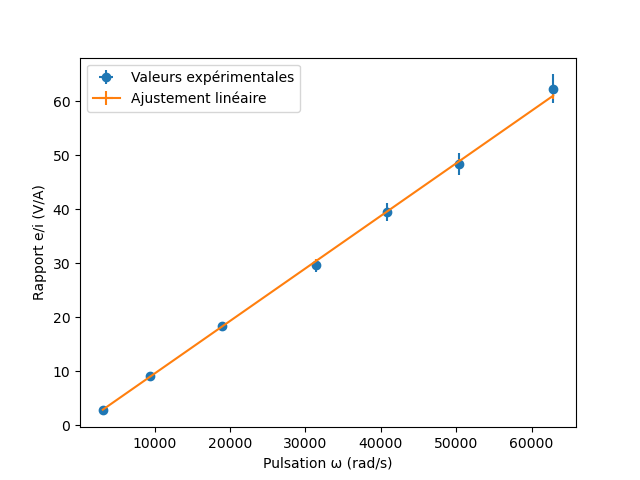
\includegraphics[width=.95\linewidth]{img/Graph_1000spires.png}
      \caption{Avec $1000$ spires}
      \label{fig:sfig1}
    \end{subfigure}%
    \begin{subfigure}{.5\textwidth}
      \centering
      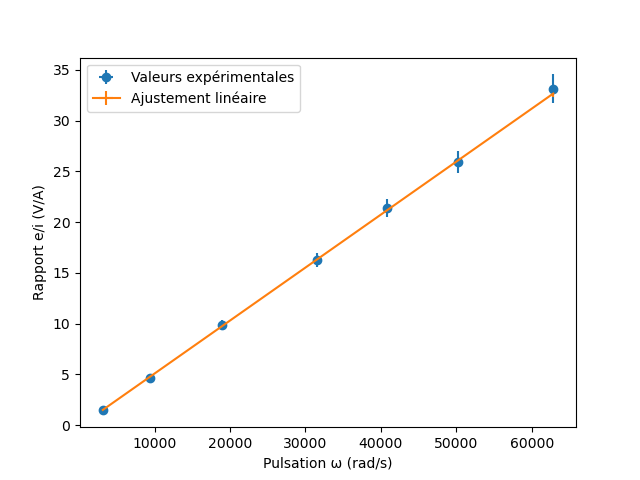
\includegraphics[width=.95\linewidth]{img/Graph_500spires.png}
      \caption{Avec $500$ spires}
      \label{fig:sfig2}
    \end{subfigure}
\end{figure}

Par régression linéaire nous obtenons $M$ d'après (\ref{eqn:relation_M}):
\begin{align}
    \text{1000 spires: } M_1 = (9.74 \pm 0.09) \times 10^{-4} V.A^{-1}.s^{-1}, b_1 = -0.16 \pm 0.07 V.A^{-1} \\
    \text{500 spires: } M_2 = (5.22 \pm 0.05) \times 10^{-4} V.A^{-1}.s^{-1}, b_2 = -0.14 \pm 0.04 V.A^{-1}
\end{align}

On remarque un premier écart à la théorie, avec une ordonnée à l'origine non nulle, ce qui n'est pas prédit car pour une fréquence nulle, le champ $\vec{B}$
ne varie plus, on ne devrait donc plus observer de f.e.m. Cependant, la présence de cette f.e.m résiduelle peut s'expliquer par la présence d'appareils et de câbles proches
générant un champ magnétique localement. On pourrait régler ce problème en installant le montage entre deux plus grandes bobines de Helmholtz de telle sorte
qu'elles compensent tous les champs magnétiques présents.

Concernant les valeurs d'inductance mutuelle $M_1, M_2$, connaissant $\alpha (d, N_H), S (a_{min}, a_{max})$ et $N$, on peut en déduire les valeurs 
théoriques de ces dernières avec $M_{th} = \alpha S N$:
\begin{align*}
  M_{th,1} = (1.06 \pm 0.05) \times 10^{-3} V.A^{-1}.s^{-1} \\
  M_{th,2} = (5.2 \pm 0.3) \times 10^{-4} V.A^{-1}.s^{-1}
\end{align*}

La valeur de $M_{th,2}$ se retrouve dans notre valeur $M_2$, cependant, $M_1$ et $M_{th,1}$ ne se retrouvent pas dans les incertitudes bien que les valeurs ne soient pas 
très éloignées. Il serait donc intéressant de répéter la mesure pour déterminer un écart-type de notre valeur de $M_1$ et vérifier si l'on retrouve $M_{th,1}$ dans l'intervalle de confiance.

Enfin, concernant le déphasage, pour le montage avec $1000$ spires, on observe un déphasage compris entre $89 \pm 0.9 ^{\circ}$ et $93.7 \pm 0.9 ^{\circ}$ et pour $500$ spires, on a 
un déphasage compris entre $90.7 \pm 1 ^\circ$ et $95.7 \pm 1 ^\circ$. On observe aucune corrélation entre déphasage et modification des paramètres, nous supposons donc 
que cet écart à la théorie est probablement une incertitude sur le temps sous-estimée, il serait préférable de réaliser un calcul de déphasage numériquement en récupérant
la liste de valeurs de $U_1$ et $U_2$ pour obtenir un décalage temporel plus précis.

Enfin, nous remarquons que pour de hautes fréquences (à partir 250kHz), le rapport $e/i$ diminue progressivement non linéairement, ce qui montre une des limites de notre modèle. En effet, nous nous sommes placés
dans l'approximation des régimes quasi stationnaires, mais cette approximation est invalide à haute fréquence.


\break
\subsection{Influence de l'orientation}
On reprend le montage expérimental, mais on oriente la bobine inductive de $1000$ spires de telle sorte à ce qu'elle face un angle $\theta$ avec l'axe des 2 bobines.
On repère l'angle à partir d'un cercle gradué, on estime ainsi l'incertitude à $\delta \theta = 5^{\circ}$. On positionne le GBF à $\nu = 3003.6 \pm 5 Hz$ et l'on relève la f.e.m
comme dans la partie précédente. On trace alors la f.e.m en fonction de $\cos \theta$ en annexe (voire figure \ref{fig:graphe_angle}):

On remarque que les pour des angles extrémaux loin de $90^{\circ}$, on obtient bien un comportement linéaire de la tension en fonction de $\cos \theta$,
cependant, plus on s'approche de l'angle $\theta = 90^{\circ}$, on observe une déviation à la théorie. Cet écart s'explique par $e(t)$ qui présente une forte
sensibilité à l'angle $\theta$ à l'approche de $90^{\circ}$, une légère variation pouvant faire doubler la mesure. Il est donc clair que notre incertitude sur la tension est sous-estimée
car ne prend pas en compte cet aspect de la mesure. De plus, le flux est dépendant du centragre de la bobine inductive, ainsi que de l'angle qui n'est pas précis dans le montage.
Il faudrait utiliser un montage capable d'orienter précisèment la bobine inductive, et de façon fixe car un expérimentateur devait maintenir manuellement la bobine, sinon les fils 
repoussaient la bobine. 

Ainsi, nous pouvons simplement affirmer que l'on observe une tension presque nulle pour un angle $\theta = 90^{\circ}$, et que la théorie prédit correctement l'aspect qualitatif de la f.e.m pour des angles faibles.
L'absence de symétrie de nos mesures ne nous permet pas de les prendre en compte pour une analyse plus en détails car l'ensemble de nos tensions pourraient être mauvaises.

\subsection{Cas d'un courant "triangulaire"}
On reprend le montage expérimental initial avec une bobine inductive à $1000$ spires, au centre des deux bobines. On passe le GBF en signal triangulaire et l'on fixe la fréquence
à $\nu = 200 \pm 1 Hz$. On observe (voir figure \ref{fig:oscillo}) bien un signal triangulaire pour $U_1$, mais la bobine inductive subit une f.e.m suivant un signal carré, et l'on remarque
que sur les ascendants du signal triangulaire, la f.e.m est négative et constante; et sur les descendants du signal triangulaire, la f.e.m est positive et constante.
Cette observation est cohérente avec la loi de Lenz-Faraday car sur un ascendant de $U_1$, on a une pente constante positive ($\frac{di}{dt} > 0$), d'où une f.e.m négative constante ($-\frac{d\Phi}{dt} \propto -\frac{di}{dt} < 0$), et inversement sur un descendant.
Fait notable, nous ne notons pas de déphasage entre les deux signaux par rapport à un signal sinusoïdal.

\section{Transformateurs de tension}
\subsection{Théorie}
Soit un circuit fermé reliant le GBF et une bobine d'inductance $L_1$, et un second circuit ouvert proche contenant une seule bobine d'inductance $L_2$.
On note $U_{GBF}$, la tension du GBF, et $U_2$ la tension aux bornes de la bobine non alimentée, on s'attend alors à avoir la relation suivante entre les deux tensions:
\begin{equation}
  \label{eqn:GBF}
  U_2 = \frac{M}{L_1}U_{GBF}
\end{equation}

\subsection{Protocole et expérimentation}
Pour vérifier la relation (\ref{eqn:GBF}), on installe 2 bobines (une de 500 spires, et une autre de 1000) que l'on relie par un noyau en U de fer
que l'on referme par un joug. On fixe la fréquence du GBF à $\nu = 1.10^3 \pm 1 Hz$ puis l'on alimente la bobine de 500 spires. Enfin, pour différentes valeurs d'amplitude du GBF, on mesure la tension aux bornes des deux bobines ainsi que le déphasage
entre les deux signaux en suivant la méthode de mesures dans la partie (\ref{section:protocole}). On repète ensuite l'opération en alimentant cette fois la bobine de 1000 spires. On s'attend à obtenir une fonction linéaire entre $U_2$ et $U_{GBF}$.

\break
On trace la tension secondaire $U_2$ en fonction de la tension primaire $U_{GBF}$, on obtient alors:
\begin{figure}[h!]
  \centering
  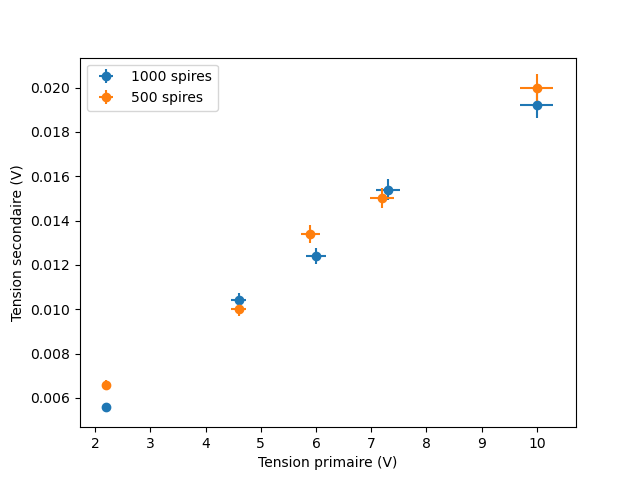
\includegraphics[width=.5\linewidth]{img/Graph_3.png}
  \caption{Tension secondaire en fonction de la fonction primaire du GBF}
  \label{fig:transformateur}
\end{figure}

On note $a_{1}, b_{1}$ les coefficients de (\ref{eqn:GBF}) lorsque la bobine de 500 spires est alimenté, et $a_{2}, b_{2}$ quand c'est la bobine de 1000 spires qui est alimenté. La régression linéaire donne:
\begin{align*}
  U_{2, 1000 \text{ spires}} = a_1 U_{GBF} + b_1, a_1 = (1.83 \pm 0.07) \times 10^{-3}, b_1 = (1.65 \pm 0.28) \times 10^{-3} V \\
  U_{2, 500 \text{ spires}} = a_2 U_{GBF} + b_2, a_2 = (1.71 \pm 0.09) \times 10^{-3}, b_2 = (2.7 \pm 0.4) \times 10^{-3} V
\end{align*}

On remarque que pour les deux montages, on retrouve ce que la théorie prédit avec la tension secondaire $U_2$ proportionnel à la tension primaire $U_{GBF}$. 
Pour le déphasage, nous observons un déphasage de $290 \pm 10 \mu s$ entre les différentes amplitudes et cela pour les deux montages. Cependant, nous ne pouvons
pas déterminer quantitativement l'exactitude de la théorie car il faudrait refaire le premier protocole dans la partie (\ref{section:protocole}) pour déterminer l'inductance mutuelle
entre les deux petites bobines.

Enfin, en ouvrant le noyau en U, nous observons une division de la tension $U_2$, ce qui signifie que l'on a une variation de flux plus faible, et lorsque l'on retire totalement le noyau,
la tension $U_2$ devient presque nulle dans les deux montages. Cela s'explique par la nature du noyau en fer doux, constitué de multiples lamelles de fer, jouant le rôle de guides d'ondes,
confinant donc le champ électromagnétique dans le noyau. Ainsi, en retirant entièrement le noyau, on déconfine le champ magnétique, réduisant le flux pouvant passer dans l'autre bobine.

\section{Conclusion}
En conclusion, nous avons réussi à montrer que la loi de Lenz prédit correctement autant qualitativement que quantitativement la force électromotrice induite 
par une variation d'un champ magnétique malgré un léger écart à la théorie quant à la prédiction de la valeur de l'inductance mutuelle, étant certainement correct à l'incertitude près
si l'on pouvait refaire l'expérience. L'influence de l'angle est vérifié pour des angles faibles, mais l'on ne peut pas en dire autant pour des angles à $90 \pm 45^\circ$. Nous avons probablement
fait des erreurs de manipulations menant à de tels résultats, il faudrait alors réaliser cette même expérience en profitant pour installer les améliorations proposées. Nous avons caractérisé
la f.e.m induite par un signal triangulaire qui est carré, qui est prédite par la loi de Lenz-Faraday. Nous avons aussi pu vérifier la relation entre la f.e.m et une bobine 
sous une tension $U_{GBF}$, prédite par la résolution des équations différentielles utilisant la loi de Lenz. Enfin, on a pu comprendre l'importance du noyau en U
de fer présent, élément important pour le confinement et la canalisation du champ magnétique d'une bobine dans l'autre, pour former un transformateur.


\break
\section*{Annexes}
\subsection{Influence de l'orientation}
\begin{figure}[h!]
  \centering
  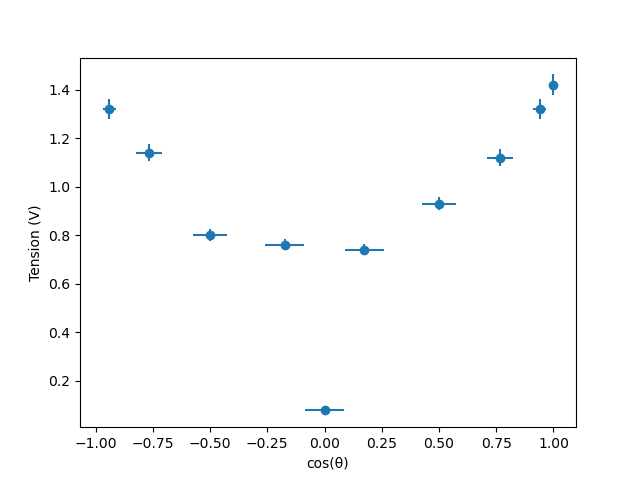
\includegraphics[width=.5\linewidth]{img/Graph_Angle.png}
  \caption{Avec $500$ spires}
  \label{fig:graphe_angle}
\end{figure}


\subsection{Cas d'un courant "triangulaire"}
\begin{figure}[h!]
  \centering
  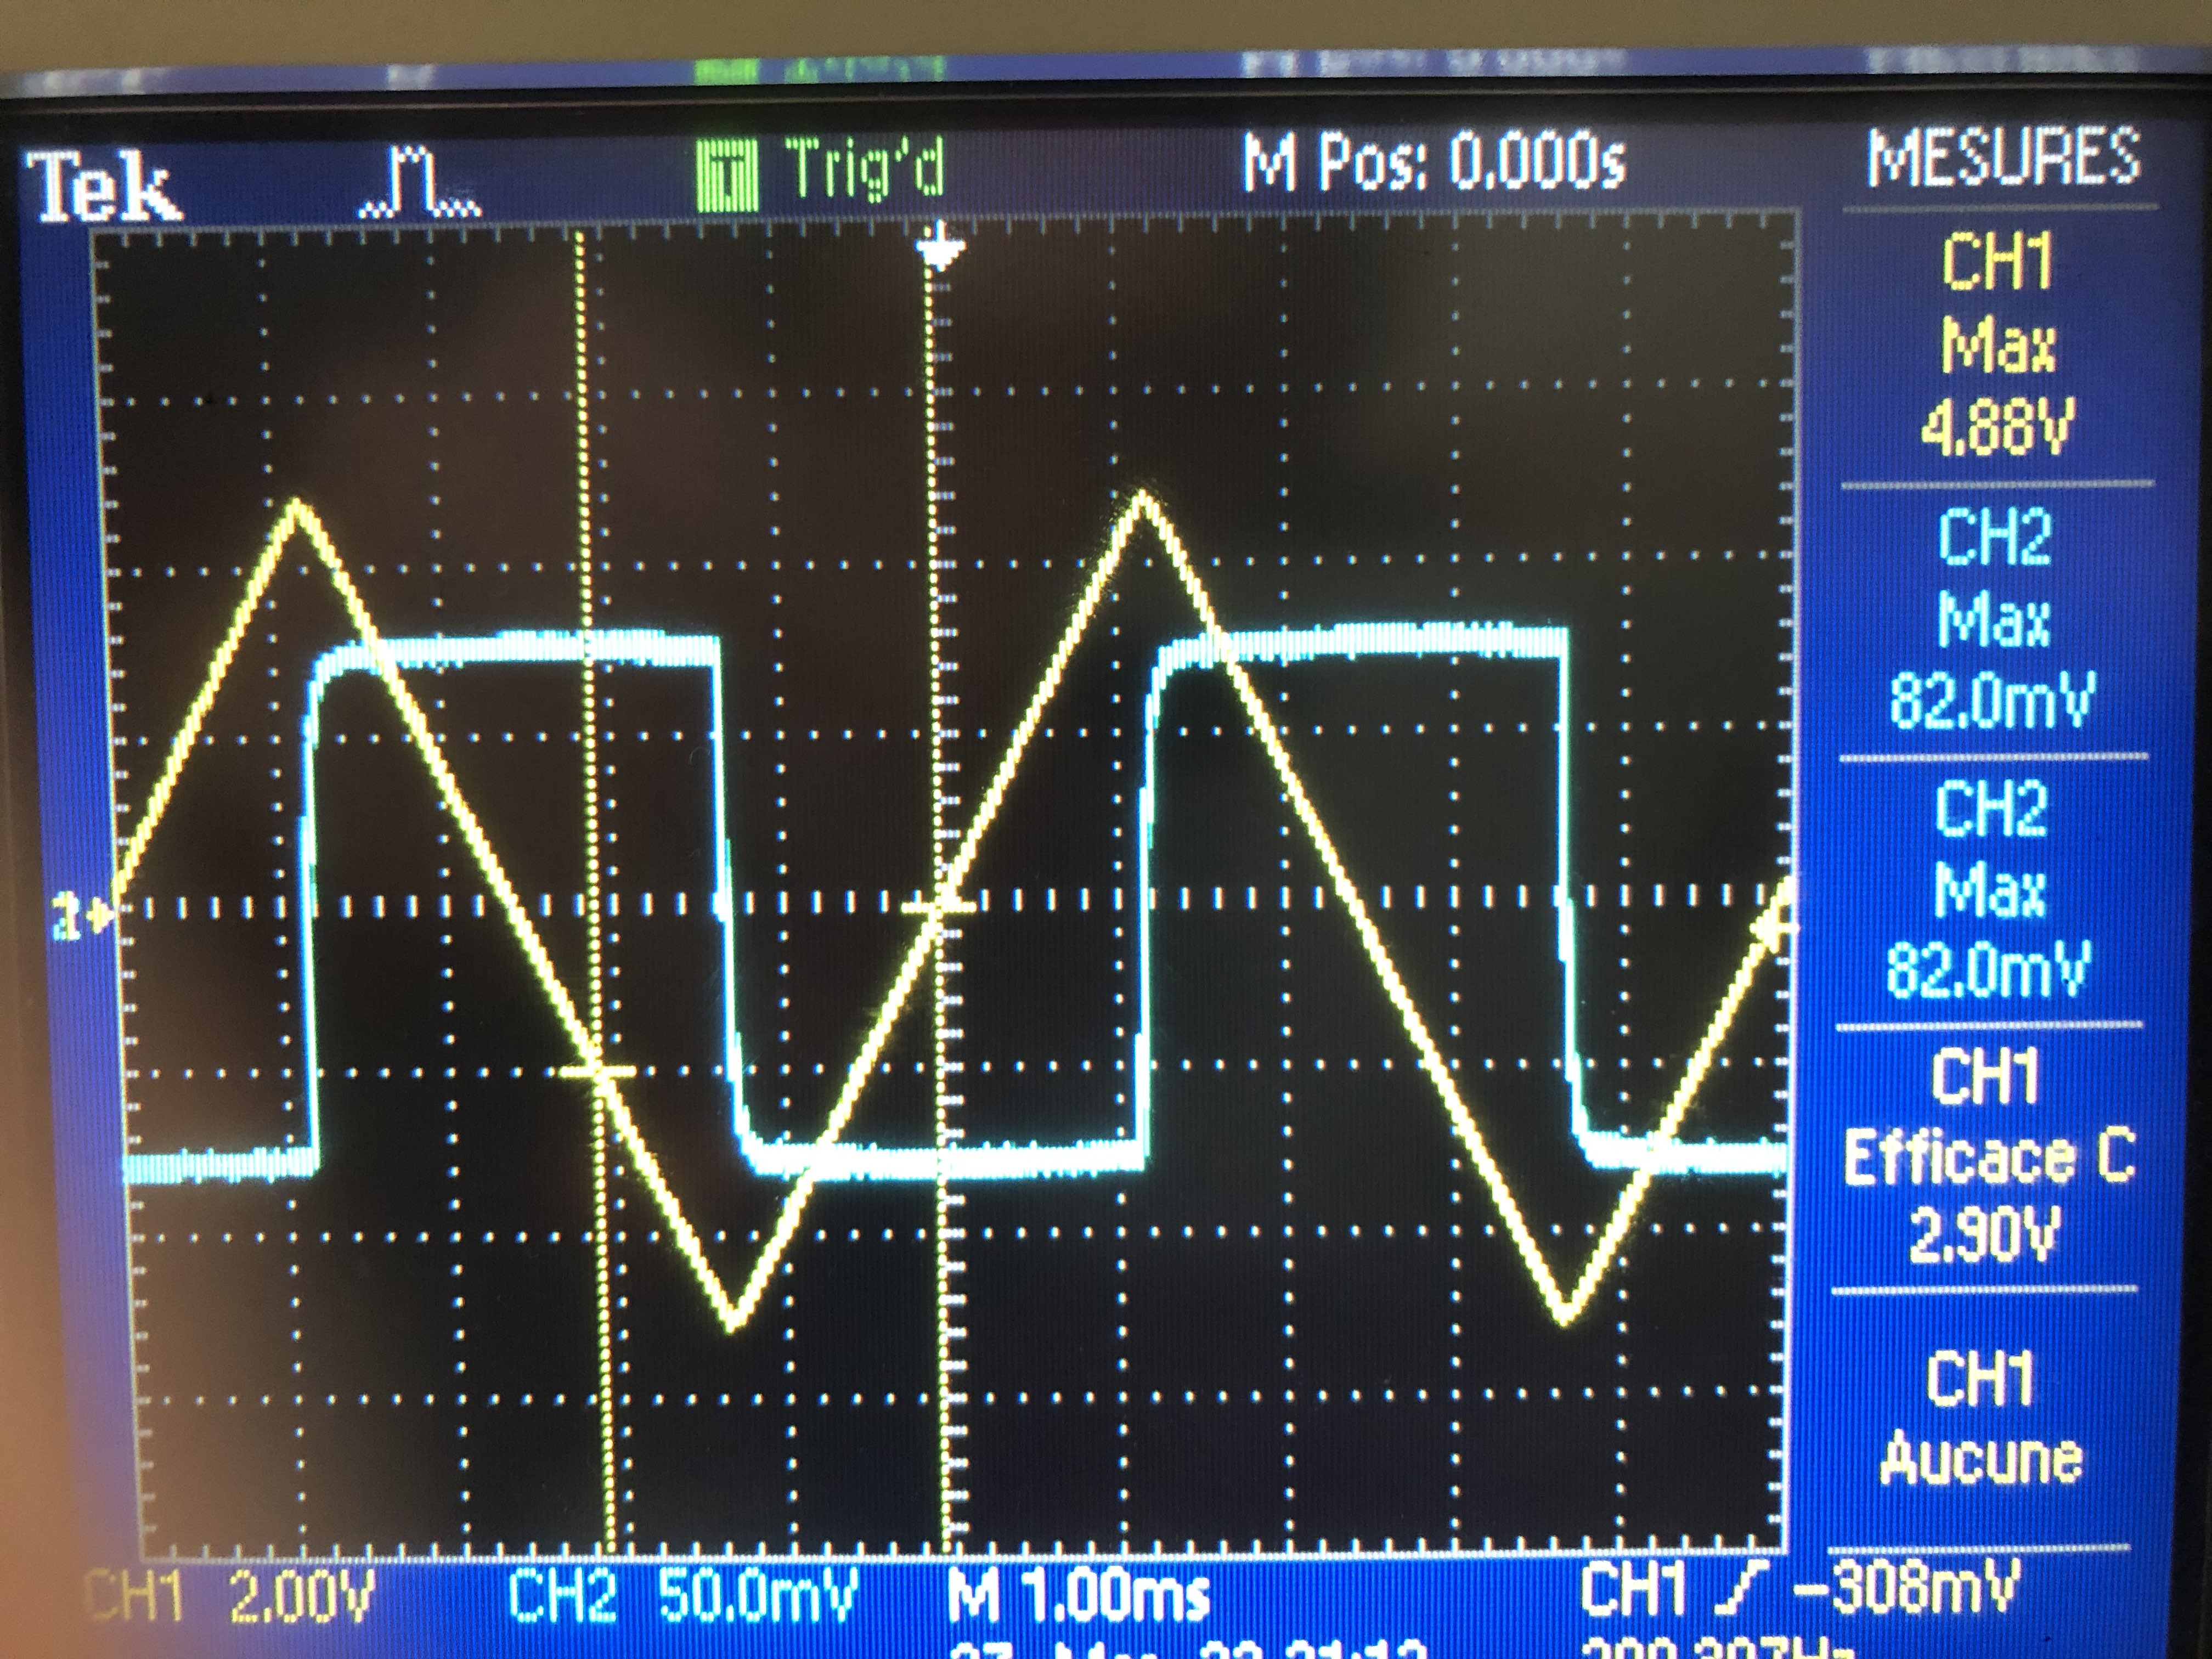
\includegraphics[width=.5\linewidth]{img/oscillo.png}
  \caption{Tension mesurée pour les deux circuits}
  \label{fig:oscillo}
\end{figure}

Le signal jaune représente $U_1$, la tension du circuit contenant la bobine de Helmholtz, et le signal bleu représente la f.e.m.


\end{document}